%% Exemple de source LaTeX pour un article soumis à TALN
\documentclass[10pt,a4paper,twoside]{article}

\usepackage[utf8]{inputenc}
\usepackage[T1]{fontenc}
\usepackage{graphicx}

% Package utilisé uniquement pour l'exemple.
\usepackage{lipsum}
\usepackage{hyperref}

% faire les \usepackage dont vous avez besoin AVANT le \usepackage{jeptaln2012} 
% add the \usepackage for you packages BEFORE the \usepackage{jeptaln2012}

\usepackage{talnrecital2013}
% Insérer les définitions de biblio en français (cf apalike-fr.bst)
\usepackage[frenchb]{babel}

\title{Bases lexicales multilingues : traitement des acronymes}

\author{Ying Zhang\up{1}\quad Mathieu Mangeot\up{1}\\
{\small  (1) GETALP-LIG, 41 rue des mathématiques  BP 53 38041 Grenoble Cedex 9\\ 
  \texttt{ying.zhang@imag.fr, mathieu.mangeot@imag.fr} \\ 
}}

\begin{document}

\maketitle

%% In an English article, use \resumeEn with 2 arguments (french title and french summary)
\resume{
La gestion des terminologies est un domaine de recherche à long terme. En particulier pour les situations compliquées comme les acronymes, la recherche n’est jamais interrompue. Dans cet article, nous parlerons de lier plusieurs termes différents à un seul référent via les notions de pivot et de prolexème. Ces notions permettent par exemple de faire le lien entre plusieurs termes qui désignent un même et unique référent : nations unies, ONU, organisation des nations unies et onusien. Il existe Jibiki, une plate-forme générique de gestion de bases lexicales permettant de gérer n’importe quel type de structure (macro et microstructure). Nous avons implémenté la notion de prolexème[…] dans la plate-forme Jibiki pour réaliser les gestions des terminologies riches comme les acronymes.
}

%% In an English article, use \abstractEn with 1 arguments (english summary)
\abstract{TALN-RECITAL2013 template (English translation of the article title)}{
The translation of the title in English is mandatory to enhance visibility of the online version of the papers in international scientific article databases (DBLP, citeseer, etc.). Here an abstract in English (max. 150 words).\\
}

\motsClefs{base lexicale multilingue, macrostructure, Jibiki, Pivax, Common Dictionary Markup, iPoLex, entrepôt de données linguistiques}
{multilingual lexical database, macrostructure, Jibiki, Pivax, Common Dictionary Markup, iPoLex, linguistic data warehouse}

%\motsClefs{Ici une liste de mots-clés en français}
%{Here a list of keywords in English}

%% Aller à la page suivante si nécessaire
%\newpage
%%================================================================
\section{Introduction}

\subsection{Situation}
L

\subsection{Intérêt}

L

\subsection{Présentation}

L

\section{Problématique}

% reprendre l'explication du cahier des charges des acronymes
% ajouter une référence à une demande industrielle de L&M.
Les liens entre les termes sont compliqués. Il existe la possibilité de lier plusieurs termes différents à un seul référent : Jean-Paul II et Karol Jozef Wojtyla en français, ou en anglais John Paul II et Karol Jozef Wojtyla. De même, certains liens évoluent avec le temps : le pape désignait Jean-Paul II en 2004 et Benoît XVI en 2012. Des pays parlant la même langue (p. ex : France et Suisse romande) peuvent également utiliser des mots différents pour le même concept. Ex : "chien renifleur" et "chien drogue". Inversement, le même terme peut désigner des concepts différents : Dans la province de langue allemande de Bolzano en Italie, le Landeshauptmann est le président du conseil provincial, avec des compétences beaucoup plus limitées que le Landeshauptmann autrichien, qui est à la tête de l'un des Etats (Land) de la fédération autrichienne.
Pour les gestions des acronymes, les liens riches sont plus répandu et plus complexe. Dans l'article introduisant la notion de Prolexème, il a été discuté qu’il y a des lexies ayant des acronymes dans certaines langues, mais pas dans d'autres. Par exemple, en français, il y a « organisation des nations unies », on peut aussi dire « Nations unies », « ONU », « onusien ». En anglais, on a « United Nations » et son acronyme « UNO ». En chinois, on a 联合国 qui est la seule lexie pour cette signification, et il n’y a pas d’acronyme. Quand on construit des ressources lexicales, comment créer les liens entre les acronymes et les mots standard ?\\
Dans les chapitres suivants, nous parlerons des idées pour résoudre les problèmes décrits ci-dessus. 

\section{Données : choix de la macrostructure}
% dans cet article, on ne détaille pas la microstructure. On l'évoquera seulement
Lors de toute discussion scientifique, il est primordial de bien s'entendre sur les termes utilisés. C'est pourquoi nous commencerons par définir les termes et concepts principaux que nous utiliserons par la suite.

Un dictionnaire est composé d'un ou plusieurs volumes reliés entre eux par des liens qui sont le plus souvent des liens de traduction. Un volume est un ensemble d'articles comportant des mots-vedette de la même langue. Un article comporte au moins un mot-vedette et le plus souvent d'autres informations (prononciation, classe grammaticale, définition, exemples, etc.). La structure des articles est appelée microstructure. L'organisation des volumes qui compose la structure d'un dictionnaire est appelée macrostructure. La macrostructure la plus simple est celle d'un dictionnaire monolingue ne comportant qu'un seul volume. Pour les dictionnaires bilingues langue A <-> langue B, on peut trouver des macrostructures avec deux volumes : un volume langue A -> langue B et un volume miroir langue B -> langue A. Ces macrostructures constituent l'essentiel des dictionnaires imprimés. L'avènement de l'outil électronique permet de s'abstraire des contraintes liées à l'impression, notamment la représentation restreinte à deux dimensions. Il est alors possible de concevoir des macrostructures plus complexes utilisant par exemple des volumes pivot. Le dictionnaire devient alors une base lexicale à plusieurs dimensions d'où il est ensuite possible d'extraire des vues spécifiques permettant de retrouver le format initial des dictionnaires imprimés.
Nous détaillerons trois macrostructures de ce type par la suite.

\subsection{Macrostructure pivot}

% utilise le concept de lexies (TST, Mel'cuk)
% présente le concept de structure pivot et d'axie
Le projet Papillon, lancé en 2000 \cite{MTMMEP00} a pour but de construire une ressource lexicale pour plusieurs langues dont au moins l'anglais, le français et le japonais. Les macrostructures bilingues traditionnelles obligeant à construire un dictionnaire par couple de langues, le nombre de dictionnaires croit de manière factorielle par rapport au nombre de langues en présence. Cette solution devient rapidement ingérable. Il fallait donc en trouver une nouvelle, un dictionnaire multilingue à structure pivot : un volume monolingue pour chaque langue et un volume pivot (ou volume interlingue) au centre regroupant les liens entre les articles \cite{GSMM01a}. La microstructure des article monolingues reprend le concept de lexie défini dans la lexicographie explicative et combinatoire \cite{MelcukClasPolguere95} issue de la théorie sens-texte. Chaque article décrit une lexie. Une lexie est une unité lexicale (ou sens de mot) qui est représentée soit par un lexème (regroupement de mots-forme), soit par une locution nominale.

Chaque lexie est reliée par un lien interlingue à une axie (ou acception interlingue). Les axies sont contenues dans le volume pivot. Chaque axie regroupe les équivalents dans plusieurs langues d'une même lexie (ou sens de mot).
Les concepts d'axie et de structure pivot ont été définis pour le projet Papillon et ensuite repris dans la norme Lexical Markup Framework \cite{Francopoulo09}.

%## illustration structure pivot et lexies/axies
%## mettre en valeur les concepts définis et harmoniser avec la partie ProAxie

\subsection{Macrostructure Pivax}

% présente le concept d'axème, de multiples volumes dans la même langue et de structure pivot à étages
La macrostructure pivot vue précédemment permet de résoudre le problème posé par une situation multilingue. Au niveau monolingue, par contre, on doit se contenter d'un seul volume pour chaque langue, ce qui constitue une limitation importante. Dans sa thèse, Hong-Thai Nguyen \cite{thèseHTN} avait le projet de construire une base lexicale avec des ressources issues de systèmes de traduction. Chaque système de traduction utilise un format qui lui est propre pour ses dictionnaires lui permettant de stocker des variables spécifiques. Si l'on veut regrouper ces dictionnaires, il n'est pas souhaitable de fusionner tous les dictionnaires de chaque langue. On peut par contre regrouper les lexies identiques D'une même langue dans un même objet. C'est le rôle des axèmes, ou acceptions monolingues.

Pour chaque langue ou espace lexical, ou aura alors un volume pour chaque système de traduction présent (Systran, Ariane, etc.) et un seul volume d'axème. Chaque lexie de chaque volume est reliée à un axème. Chaque axème est à son tour relié à une axie dans le volume pivot central.
Cette structure ainsi constituée est une structure pivax ou structure pivot à étages \cite{MMHTN09}. Elle peut être utilisée également pour gérer différentes version d'un même volume dans un espace lexical.
%## illustration structure Pivax

\subsection{Macrostructure ProAxies}

% utilise les concepts présentés précédemment (structure pivot à étages, multiples volumes dans la même langue, lexies, axies, axemes)
% utilise le concept de prolexème (au même niveau que les axèmes)
% présente le concept de proaxie
Cette macrostructure a pour but de résoudre le problème de faire le lien entre plusieurs termes qui désignent un même et unique référent. Pour les gestions des acronymes, les liens riches sont plus répandu et plus complexe. Dans l'article introduisant la notion de Prolexème […], il a été discuté qu’il y a des lexies ayant des acronymes dans certaines langues, mais pas dans d'autres. Par exemple, en français, il y a « organisation des nations unies »\footnotemark[1], on peut aussi dire « Nations unies », « ONU », « onusien ». En anglais, on a « United Nations » et son acronyme « UN ». En chinois, on a « 联合国 » qui est la seule lexie pour ce sens, et il n’y a pas d’acronyme. Quand on construit des ressources lexicales, comment créer les liens entre les acronymes et les mots de définition ? \\
\footnotetext[1] {Nous avons repris exactement la terminologie français de Prolexbase et les concepts.}
Donc, la macrostructure de la gestion des acronymes faudra nous permettre de 
\begin{itemize}
\begin{itemize}
\item gérer les liens  plus complexe et
\item gérer les multiples volumes dans la même langue. 
\end{itemize}
\end{itemize}
Pour implémenter la gestion des acronymes, nous avons proposé une nouvelle macrostructure avec deux notions: ProAxie et ProLexème. Nous avons certainement besoin des conceptions d’Axie [..] et de Lexie [...]. \\
\\
\textbf{ProLexème}\\
Il y a un seul volume de prolexème pour chaque langue. Dans ce volume, les prolexèmes regroupent les lexies. Les liens bidirectionnels entre les lexies et leurs prolexèmes sont marqués avec une étiquette (alias, acronyme, définition, etc.). Un sens lexical est une entrée de prolexème qui lie les lexies différentes de ce même sens. \\
Par exemple, l’entrée de prolexème est « fr.organisation\_des\_nations\_unies.1 » qui lie l’entrée de lexie 
\begin{itemize}
\begin{itemize}
\item « ONU » avec une étiquette « acronyme »
\item « nations unies » avec une étiquette « alias »
\item « onusien » avec une étiquette « alias »
\item « organisation des nations unies » avec une étiquette « définition ».
\end{itemize}
\end{itemize}
\quad  \\
\textbf{ProAxie}\\
Il y a un seul volume de proaxie dans un dictionnaire. Les proaxies regroupent les prolexèmes de langues différentes dans un même sens. Par exemple, un dictionnaire trilingue : français, anglais et chinois. L’entrée de proaxie « proaxie.united\_nations.1 » lie avec 
\begin{itemize}
\begin{itemize}
\item l’entrée « fra.organisation\_des\_nations\_unies.1 » du volume des prolexèmes français et 
\item l’entrée « eng.united\_nations.1 » du volume des prolexèmes anglais et
% verifie les choinois s'ils affichent correctement
\item l’entrée « zho.联合国.1 » du volume des prolexèmes chinois.
\end{itemize}
Les liens entre l'entrée de proaxie et les entrées de prolexèmes sont bidirectionnels.\\
\\
\textbf{Conception globale}\\
Dans cette macrostructure, nous avons deux couches : une couche basique et une couche « Pro ».  Dans la couche basique, nous avons deux types de volume : volume des lexies et volume des axies. Dans la couche « Pro », nous avons également deux types de volume : volume des prolexèmes et volume des proaxies.
Grâce au volume d’axie, nous pouvons faire les liens entre les lexies exactement correspondus, comme l’acronyme français « ONU » lie avec l’acronyme anglais « UN ». Grâce à la couche « PRO »,  nous pouvons proposer les lexies des langues cibles de même sens.  Voir le figure 1 - « Exemple de ProAxie ».\\
\begin{figure}[htbp] 
\begin{center} 
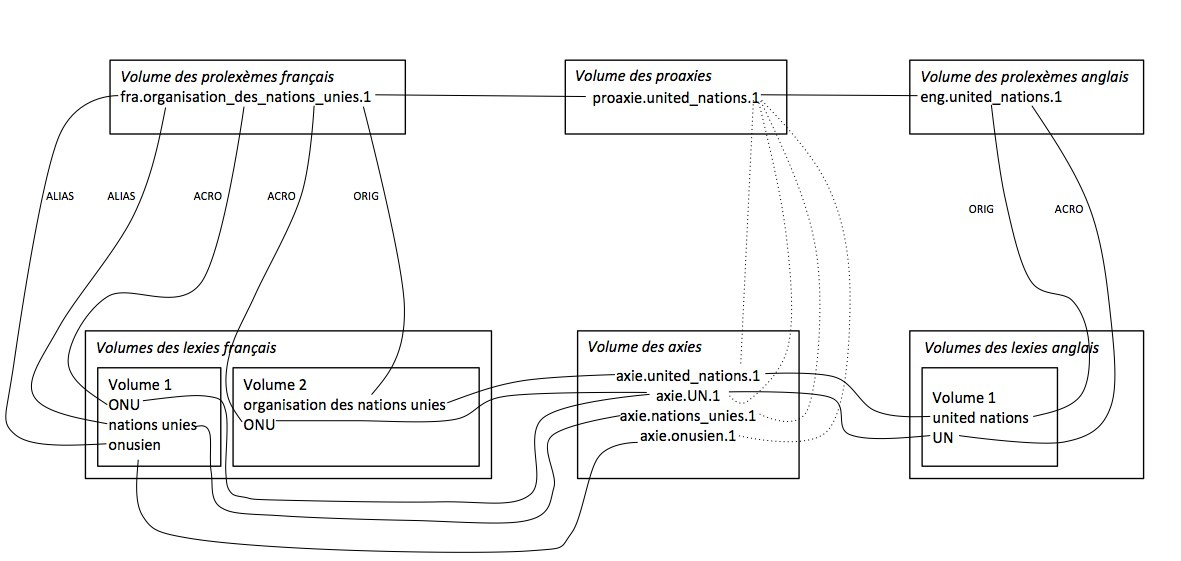
\includegraphics[width=14cm]{images/proaxie_2-etages.jpg}
\end{center} 
\caption{Exemple de ProAxie} \label{image} \
\end{figure}
La notion d’étiquette a pour but de proposer les meilleures traductions. Par exemple, le japonais « 国際連合 » est la lexie de sens de « Organisation des nations unies », son acronyme est « 国連 » comme le table 1 - « Exemple de quatre langues pour le sens "Organisation des nations unies" ». Cet acronyme utilise le premier et le troisième caractère de kanji, ce n’est pas utilisé les initiales de lexie de définition. Il existe sans-doute une langue qui a deux acronymes, un correspond à l’acronyme initiales, un autre correspond à la sélection de caractère ou de mot.  Donc, nous avons décidé de ne pas lier ces deux types acronymes avec un même axie. Voir le figure 2 - « Liens entre les lexies et les axies » \\
\begin{table}[!h]
\centering
	\begin{tabular}{|l|l|l|l|l|}
	\hline
	\textbf{Langue} & \textbf{Anglais} & \textbf{Français} & \textbf{Chinois} & \textbf{Japonais} \\
	\hline
	\textbf{Définition} & united nations & organisation des nations unies & 联合国 & 国際連合 \\
	\hline
	\textbf{Acronyme} & UN & ONU & & 国連 \\
	\hline
	\textbf{Alias} & & onusien, nations unies & &  \\
	\hline
	\end{tabular}
\caption{ Exemple de quatre langues pour le sens "Organisation des nations unies" }\label{table}
\end{table}

\begin{figure}[htbp] 
\begin{center} 
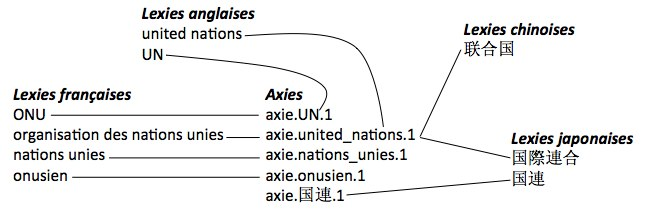
\includegraphics[width=14cm]{images/lexies-axies.jpg}
\end{center} 
\caption{Liens entre les lexies et les axies} \label{image} \
\end{figure}

Quand on cherche les liens de « ONU » de français vers l’anglais,  vers le japonais et vers le chinois. Nous avons proposé trois niveaux de traduction :\\

\begin{itemize}
\begin{itemize}
\item Vers l’anglais : ONU->UN. Le système trouve une lexie directe par le volume des axies. C’est le \textbf{premier niveau} de traduction.
\item Vers le japonais : ONU->国連. Le système cherche le lien dans le volume des prolexèmes français avec l’étiquette « Acro ». Puis il trouve le lien dans proaxies, ensuite il suit le lien de prolexème japonais, enfin il arrive le volume des lexies japonais, et il trouve une lexie avec l’étiquette « Acro ». Donc la lexie proposée du \textbf{deuxième niveau} de langue cible est cet acronyme.  Le deuxième niveau de traduction toujours comprend le premier niveau de traduction.
\item Vers le chinois : ONU->联合国.  Le système trouve les lexies par prolexeme et proaxie sans étiquette. Ces lexies proposées est le \textbf{troisième niveau}. Le troisième niveau de traduction comprend le premier et le deuxième niveau de tradcution.
\end{itemize}
\end{itemize}
La quantité de lexie de résultat est augmentée suivant les niveaux de traduction de haut vers bas. Nous avons également utilisé l’exemple de « ONU » comme la table 2 - « Trois niveaux de traduction ».\\

\begin{table}[!h]
\centering
	\begin{tabular}{|l|l|l|l|}
	\hline
	\textbf{} & \textbf{Premier niveau} & \textbf{Deuxième niveau} & \textbf{Troisième niveau} \\
	\hline
	\textbf{Français} & UN & UN & UN, United Nations \\
	\hline
	\textbf{Japonais} &  & 国連 &国連, 国際連合 \\
	\hline
	\textbf{Chinois} & & &联合国  \\
	\hline
	\end{tabular}
\caption{ Trois niveaux de traduction }\label{table}
\end{table}



Dans certaines situations, une base lexicale (un dictionnaire) a plusieurs volumes dans une seule langue. Par exemple, il y a plusieurs versions d’édition. Ou la ressource lexicale est créé par les système de TA, alors il existe un volume de Systran, un volume de Google, un volume d’IATE, etc.. Notre macrostructure permet de gérer multivolume dans une langue. Voir la figure 3 « macrostructure de proaxie ».\\
\begin{figure}[htbp] 
\begin{center} 
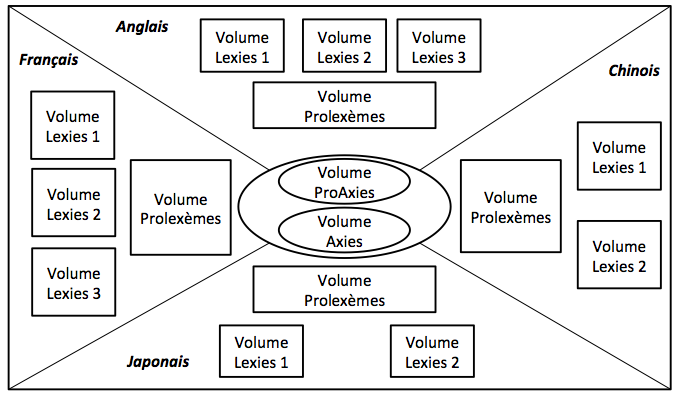
\includegraphics[width=12cm]{images/proaxie.png}
\end{center} 
\caption{Macrostructure de ProAxie} \label{image} \
\end{figure}

\section{Outils nécessaires : plateformes de manipulation}

\subsection{Plateforme Jibiki v1}

% parle des différents outils existants : tswanelex, DPC, voir
\cite{MMCE11}
% présente la plateforme : CDM et table d'index, édition générique, opensource, licence GPLv3, dispo publiquement et gratuitement sur ligforge en SVN, sert pour de multiples projets
%## illustration CDM
Pour implémenter la macrostructure de ProAxie, nous avons choisi la plat-forme Jibiki. Elle permet la construction de sites web de communauté dédiées à la constructions de bases lexicales multilingues. Cette plate-forme a été développée principalement par Mathieu Mangeot et Gilles Sérasset […]. Cette plate-forme est utilisée dans divers serveurs (projet LexALP, projet Papillon, projet GDEF, etc.). Elle est un projet de source ouvert. Nous pouvons télécharger gratuitement sur ligforge en SVN. Avec cette plate-forme, on peut faire les manipulations des import, export, édit, modification et recherche de base lexicale. On peut aussi gérer les contributions. \\
C’est une plate-forme générique, elle permet de traiter presque toutes les ressources lexicales de type XML en utilisant les stratégies de microstructure et macrostructure. La microstructure est la structure des entrées. On utilise des pointeurs CDM (Common Dictionary Markup) […] pour gérer n’importe quel type de microstructure sans la modifier. Cette structure est stockée dans un fichier de métadonnées sous forme XML. On réalise les programmes d’import des chemins Xpath des éléments correspondant à des éléments de CDM dans le fichier XML à importer. Voir le figure 4 - « Exemple de CDM ». \\
\begin{figure}[htbp] 
\begin{center} 
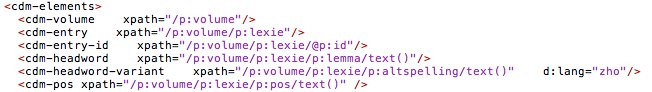
\includegraphics[width=14cm]{images/CDM.jpg}
\end{center} 
\caption{Exemple de CDM} \label{image} \
\end{figure}

% explique les limitations : pas de liens entre plusieurs volumes différents, macrostructures complexes (pivot, pivax, etc.) codées en dur, difficultés de création de méta-données


\cite{MMAC06}

\subsection{Gestion des données et méta-données : iPoLex}

% explique le concept d'entrepôt de données
% génération assistée des méta-données

Une fois la première version de Jibiki réalisée, nous nous sommes rendus compte d'un autre problème soulevé par les ressources : que faire des fichiers de données brutes au format textuel avant importation et après exportation de la plate-forme ? 
De plus, la rédaction de fichiers XML de méta-données décrivant chaque ressource est très délicate et réservée à des informaticiens avertis.
La gestion des différentes versions d'une même ressource pose également problème.
Enfin, les ressources au format textuel peuvent être utilisées directement par d'autres applications. Il convient donc d'organiser leur stockage dans de bonnes conditions.

L'idée s'est alors imposée de concevoir un entrepôt de données lexicales permettant de stocker les données brutes au format textuelles ainsi que de définir les métadonnées d'une nouvelle ressource à l'aide d'une interface. Ce projet, nommé iPoLex avait comme objectif d'être simple et rustique. L
%## rechercher l'origine du nom du projet dans t7o.

L'entrepôt est accessible par le Web. Les interfaces sont programmées en PHP sans connexion à une base de données. Toutes les informations sont stockées dans des fichiers texte. 
La page d'accueil affiche la liste des ressources disponibles et permet d'effectuer différents tris (format, langue source, langues cibles, etc).
%## illustration liste des ressources

L'ajout d'une nouvelle ressource se fait en trois étapes : d'abord la description de la ressource avec ses méta-données (langues source et cibles, domaine, auteur, date de création, format, taille des fichiers texte, etc.) puis, pour chaque volume de la ressource, la description de ses métadonnées (langue source, nombre de mots-vedette, version, etc.) ainsi que celle des pointeurs CDM permettant d'indexer le volume après importation dans la base Jibiki.
La description des ressources se termine par la création d'un répertoire sur le serveur et la génération de fichiers de méta-données.
%## illustration saisie de métadonnées
La dernière étape est celle du téléversement des fichiers de données sur le serveur. Pour cela, l'entrepôtpeut se monter comme répertoire distant grâce au protocole WebDAV.
Une fois les fichiers de données téléversés sur le serveur, l'import dans une plate-forme Jibiki se fait très facilement en indiquant dans l'interface de Jibiki l'URL du fichier de méta-données de la ressource à importer.

Nous prévoyons d'étendre ce concept d'entrepôt de données à celui d'entrepôt de services. En effet, pour la plupart des ressources stockées dans l'entrepôt, il existe des services associés comme par exemple des moulinettes de conversion d'un format à un autre. Ces scripts sont en général prévus pour une version particulière des données. S'ils ne sont pas documentés précisément et stockés avec les données, il est très difficile, voire impossible de réexécuter les processus divers associés aux données.

%## illustration répertoire distant dictionnaires (optionnel)

\subsection{Gestion des liens riches : extension Jibiki-Pivax}

% explique la nouvelle gestion des liens riches : 
% liens : volume de destination, poids, type (axi, final), langue, étiquette libre, etc. 
% table de liens séparée
% algorithme de collecte des liens dans DictionariesFactory.java (expandResults)
% algorithme de construction du résultat : parcours montant vers les axies puis descendant vers les lexies cibles

\section{Résultats préliminaires}

% montre les résultats de recherche pour différents scénarios
Nous avons divisé trois niveaux de traduction pour afficher les résultats de recherche dans Jibiki: 1er – traduction directe par axie, 2ème – traduction par prolexème et proaxie avec la même étiquette, 3ème – traduction par prolexème et proaxie sans étiquette.  Pour faciliter à lire, nous avons décidé : 
\begin{itemize}
\begin{itemize}
\item d’afficher l’étiquette, la langue et le mot-vedette dans le 1er et le 2ème niveaux, 
\item d’afficher tous les détails dans le 3ème niveau, y compris les lexies de la langue source
\item de ne pas afficher la traduction dans le 2ème niveau si elle a déjà trouvé et est déjà affichée dans 1er niveau,
\end{itemize}
\end{itemize}

% scénario 1 : montre si une axie est dispo ONU => ONU en chinois 
\subsection{scénario 1 :  UN d'anglais vers toutes les langues}

\begin{table}[!h]
\centering
	\begin{tabular}{|p{1cm}|p{1.8cm}|p{0.5cm}|p{1cm}|p{1cm}|p{1.8cm}|p{1cm}|p{1cm}|p{1cm}|}
	\hline
	\textbf{Niveau} & \multicolumn{4}{l|}{\textbf{ Lexies trouvés par théories}}&\multicolumn{4}{l|}{\textbf{Lexies affichées par interface}} \\
	\cline{2-9}
	&\textbf{Fra} & \textbf{Eng} & \textbf{Zho} & \textbf{Jpn} & \textbf{Fra} & \textbf{Eng}  & \textbf{Zho} & \textbf{Jpn} \\
	\hline
	\textbf{1} & ONU &  &  &  & ONU &  &  &   \\
	\hline
	\textbf{2} & ONU &  &  &国連&  &  &  &国連 \\
	\hline
	\textbf{3} & \raggedright ONU, Nations unies, onusien, Organisation de nations unies & \raggedright  & \raggedright 联合国 & \raggedright 国際連合, 国連 & \raggedright ONU, Nations unies, onusien, Organisation de nations unies  & \raggedright UN, United Nations &  \raggedright 联合国 & 国際連合, 国連 \\
	\hline
	\end{tabular}
\caption{ Trois niveaux de traduction et affichage : UN d'anglais vers toutes les langues}\label{table}
\end{table}

\begin{figure}[htbp] 
\begin{center} 
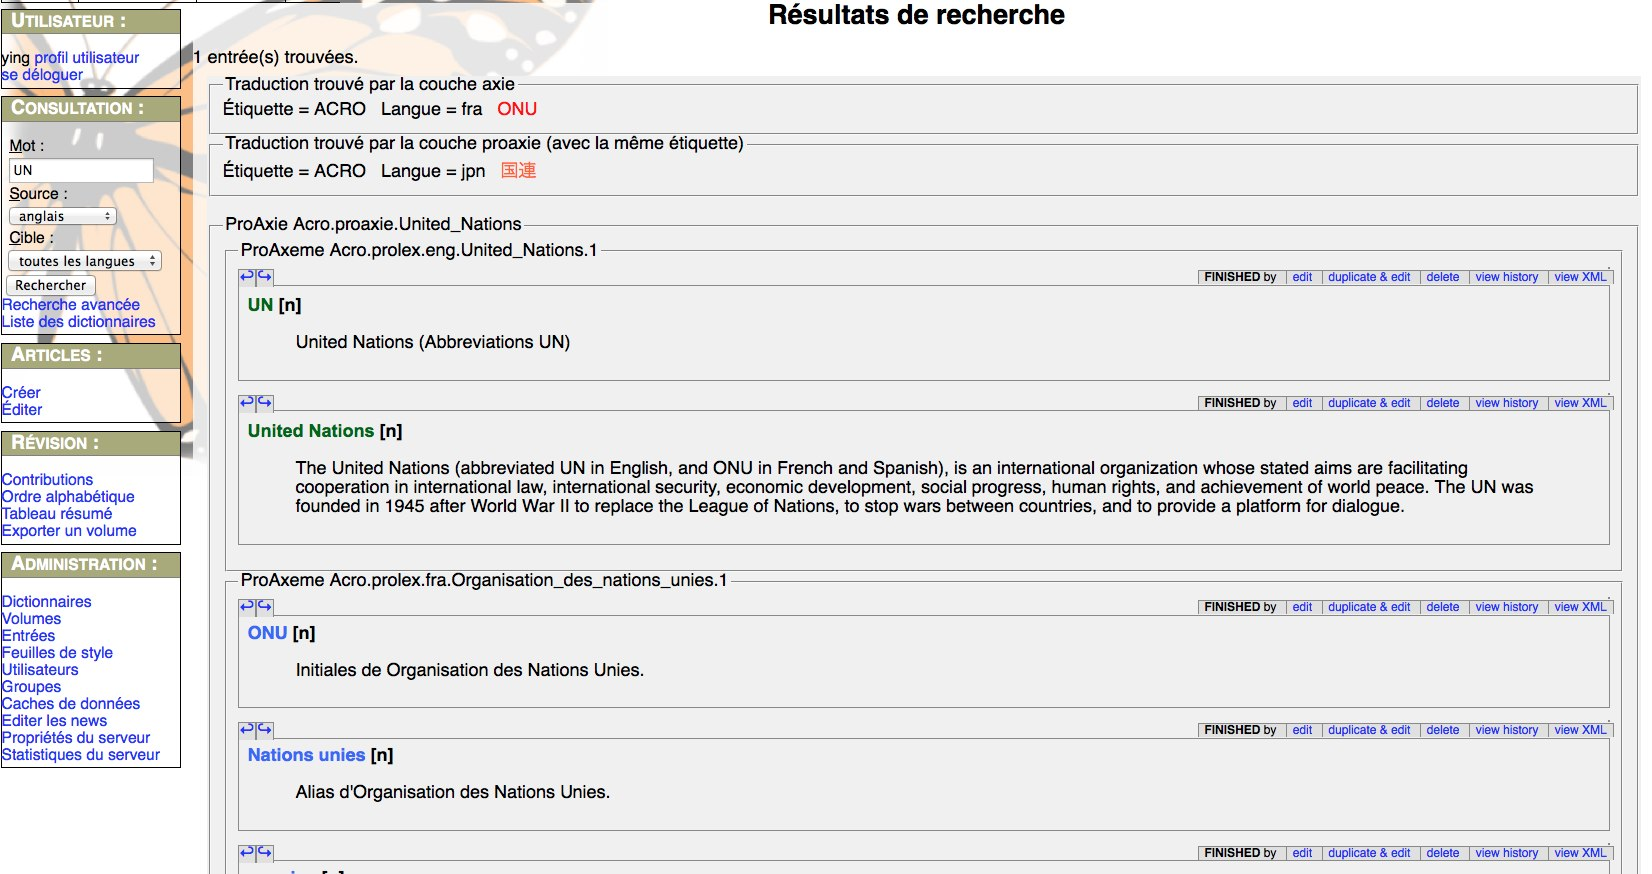
\includegraphics[width=14cm]{images/scenario1-1.jpg}
\end{center} 
\caption{UN d'anglais vers toutes les langues} \label{image} \
\end{figure}

\begin{figure}[htbp] 
\begin{center} 
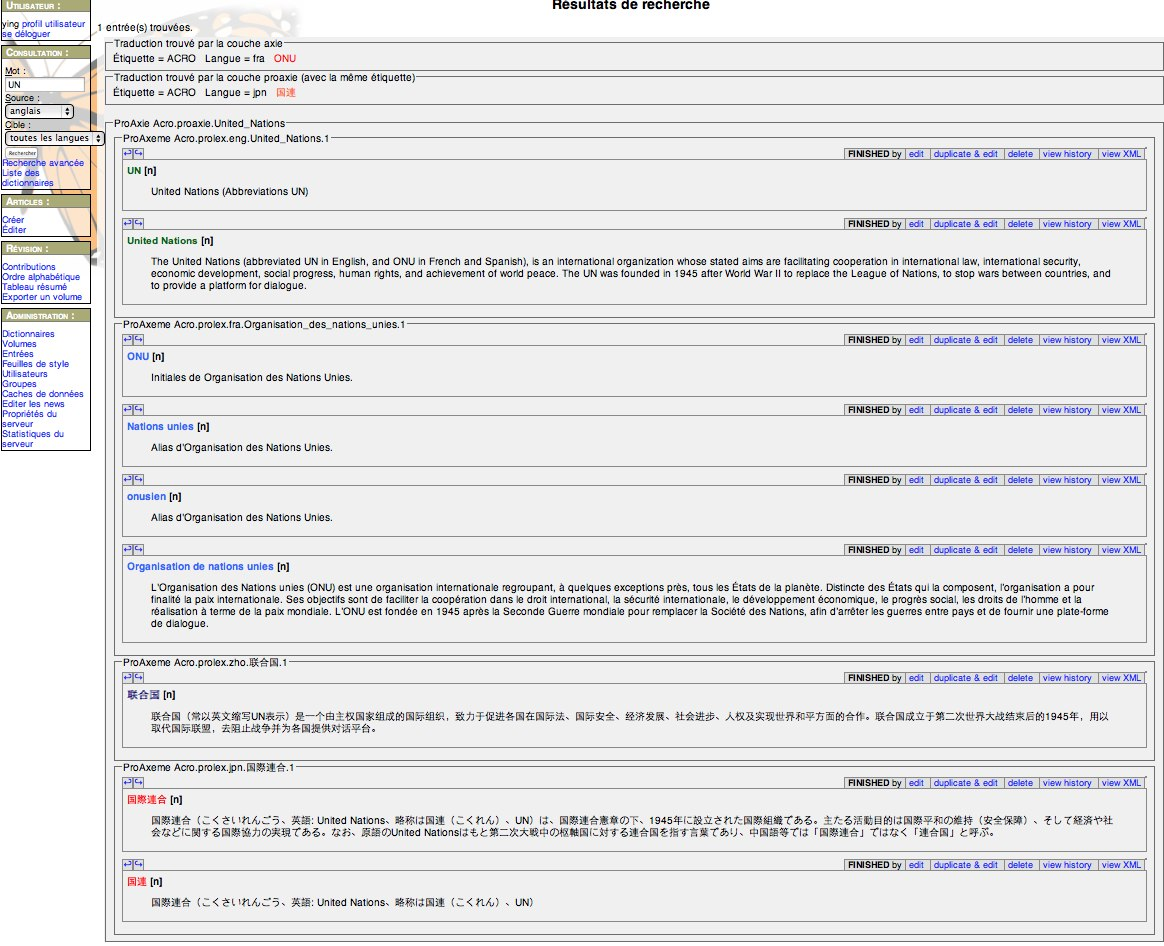
\includegraphics[width=14cm]{images/scenario1-2.jpg}
\end{center} 
\caption{Affichage complet - UN d'anglais vers toutes les langues} \label{image} \
\end{figure}

% scénario 2 : montre s'il n'y a pas d'axie de dispo, on passe par la proaxie et on utilise l'étiquette (label) Organisation des Nations Unies => United Nations
\subsection{scénario 2 :  国連 de japonais vers toutes les langues}

\begin{table}[!h]
\centering
	\begin{tabular}{|p{1cm}|p{1.8cm}|p{1cm}|p{1cm}|p{0.5cm}|p{1.8cm}|p{1cm}|p{1cm}|p{1cm}|}
	\hline
	\textbf{Niveau} & \multicolumn{4}{l|}{\textbf{ Lexies trouvés par théories}}&\multicolumn{4}{l|}{\textbf{Lexies affichées par interface}} \\
	\cline{2-9}
	&\textbf{Fra} & \textbf{Eng} & \textbf{Zho} & \textbf{Jpn} & \textbf{Fra} & \textbf{Eng}  & \textbf{Zho} & \textbf{Jpn} \\
	\hline
	\textbf{1} &  &  &  &  &  &  &  &   \\
	\hline
	\textbf{2} & ONU & UN &  & & ONU & UN &  &国連 \\
	\hline
	\textbf{3} & \raggedright ONU, Nations unies, onusien, Organisation de nations unies & \raggedright UN, United Nations & \raggedright 联合国 & & \raggedright ONU, Nations unies, onusien, Organisation de nations unies  & \raggedright UN, United Nations &  \raggedright 联合国 & 国際連合, 国連 \\
	\hline
	\end{tabular}
\caption{Trois niveaux de traduction et affichage : 国連 de japonais vers toutes les langues}\label{table}
\end{table}

\begin{figure}[htbp] 
\begin{center} 
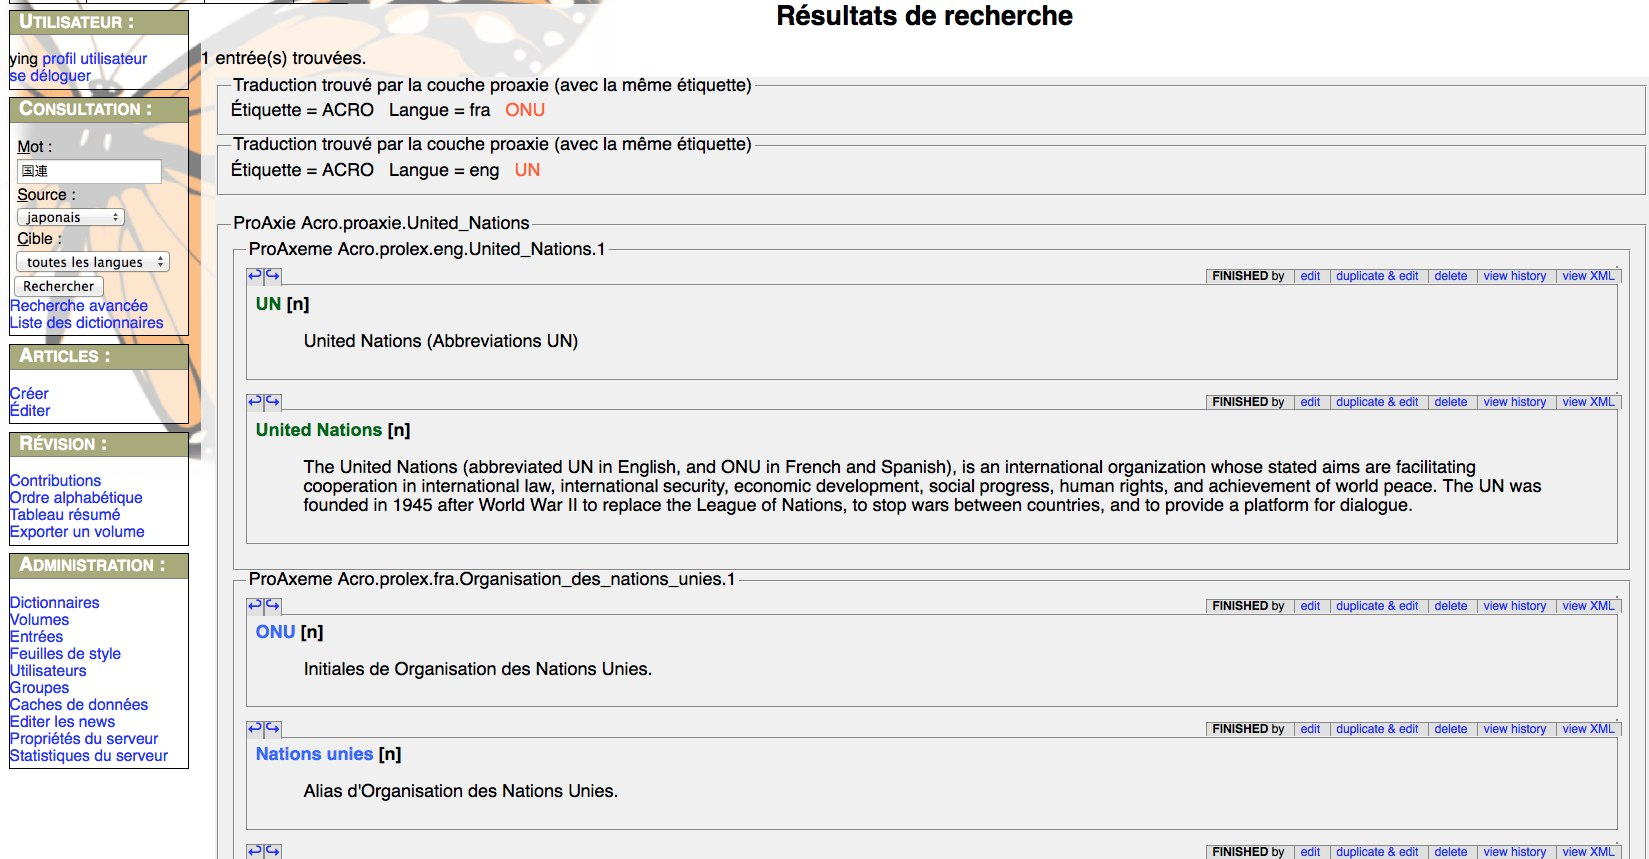
\includegraphics[width=14cm]{images/scenario2.jpg}
\end{center} 
\caption{Affichage complet - UN d'anglais vers toutes les langues} \label{image} \
\end{figure}


% scénario 3 : montre s'il n'y a pas d'axie de dispo et pas d'étiquette correspondante. On utilise seulement la proaxie : Trouver un exemple avec un acronyme dans une langue et pas dans une autre (onusien vers chinois et vers anglais)
\subsection{scénario 3 :  onusien de français vers toutes les langues}
\begin{table}[!h]
\centering
	\begin{tabular}{|p{1cm}|p{1.8cm}|p{1cm}|p{1cm}|p{0.5cm}|p{1.8cm}|p{1cm}|p{1cm}|p{1cm}|}
	\hline
	\textbf{Niveau} & \multicolumn{4}{l|}{\textbf{ Lexies trouvés par théories}}&\multicolumn{4}{l|}{\textbf{Lexies affichées par interface}} \\
	\cline{2-9}
	&\textbf{Fra} & \textbf{Eng} & \textbf{Zho} & \textbf{Jpn} & \textbf{Fra} & \textbf{Eng}  & \textbf{Zho} & \textbf{Jpn} \\
	\hline
	\textbf{1} &  &  &  &  &  &  &  &   \\
	\hline
	\textbf{2} &  &  &  & &  &  &  &連 \\
	\hline
	\textbf{3} &  & \raggedright UN, United Nations & \raggedright 联合国 &\raggedright 国際連合, 国連 & \raggedright ONU, Nations unies, onusien, Organisation de nations unies  & \raggedright UN, United Nations &  \raggedright 联合国 & 国際連合, 国連 \\
	\hline
	\end{tabular}
\caption{Trois niveaux de traduction et affichage : onusien de français vers toutes les langues}\label{table}
\end{table}
\begin{figure}[htbp] 
\begin{center} 
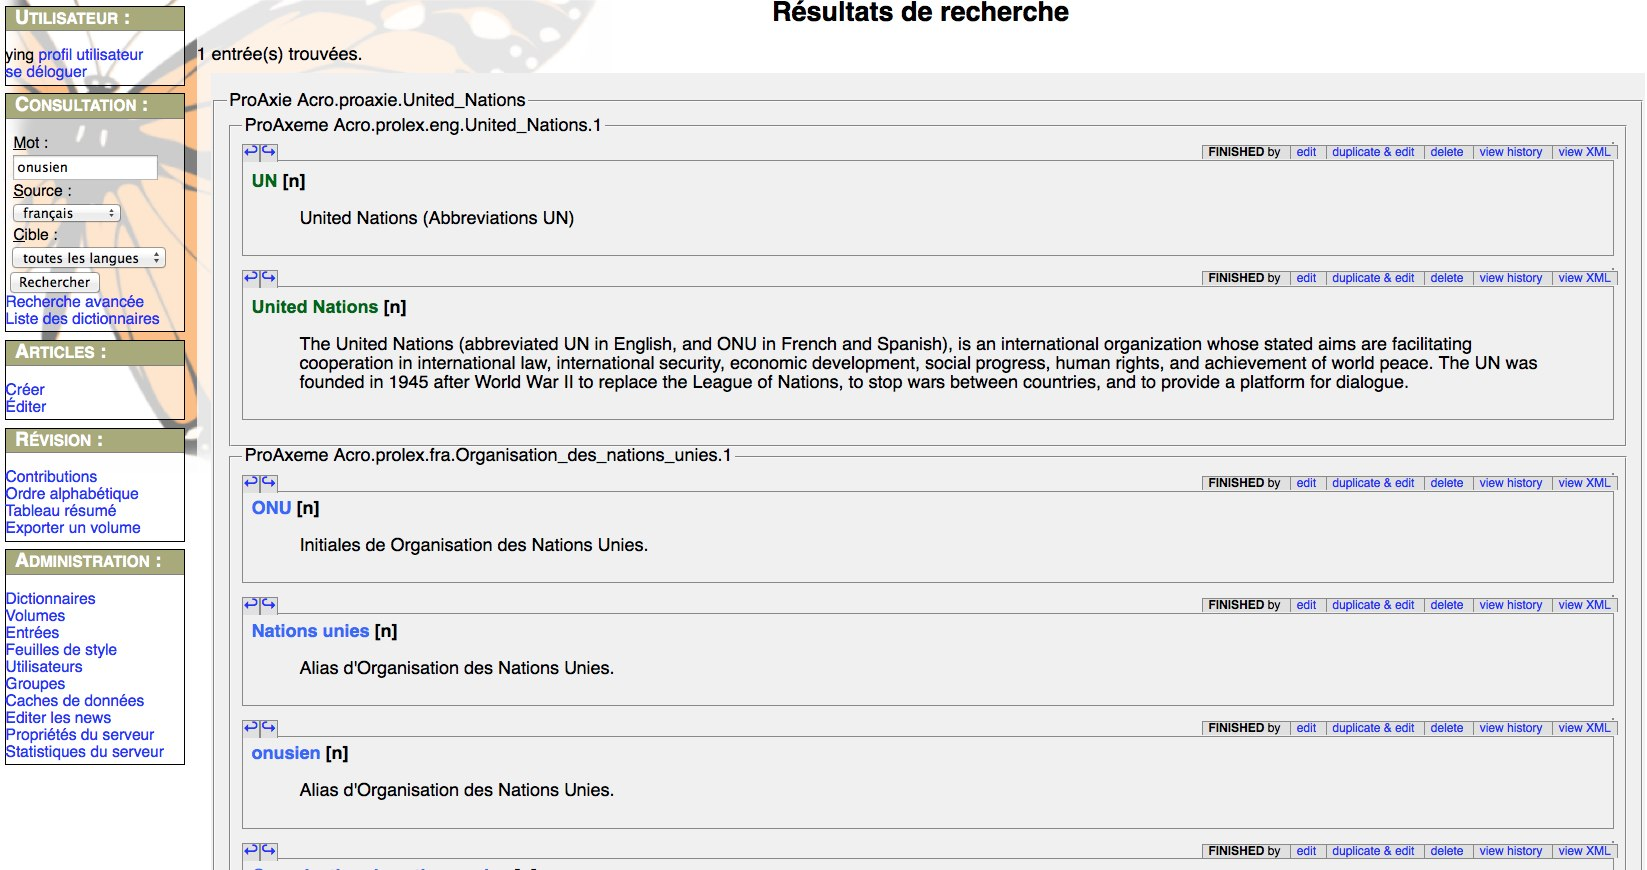
\includegraphics[width=14cm]{images/scenario3.jpg}
\end{center} 
\caption{Affichage complet - UN d'anglais vers toutes les langues} \label{image} \
\end{figure}
\section{Conclusion}

L

% à effacer à la fin
\section{Exemples à effacer à la fin}

\begin{itemize}
\item Une liste à puce
\item avec plusieurs lignes
\item pas trop espacées... 
\end{itemize}

\begin{enumerate}
\item Une liste numérotée
\item où le 2. succède, étrangement, au 1.
\item et le trois, au deux... (ce serait pas ambigu cela ?)
\end{enumerate}

\subsubsection{Figures et tables}

Les figures et les tables seront centrées sur la page avec une légende située en dessous. La légende contiendra le mot clé figure (ou table) en petite capitale, suivi du numéro de la figure ou de la table (numéros indépendants). La figure \ref{image} et la table \ref{table} en sont un exemple. Les équations peuvent figurer "en ligne" ou centrées sur la page, sans légende. Un numéro de renvoie peut figurer à droite de l'équation pour permettre les références dans le texte.

\begin{table}[!h]
\centering
	\begin{tabular}{|c|p{4cm}|}
	\hline
	Un tableau&\\
	\hline
	&Les cellules ainsi que le tableau sont centrés\\
	\hline
	\end{tabular}
\caption{Un tableau}\label{table}
\end{table}

\begin{figure}[htbp] 
\begin{center} 

\includegraphics{images/atala.png}
\end{center} 
\caption{Une image comme figure} \label{image} \
\end{figure}
Paragraphe facultatif

%%================================================================
%% Note : si l'on préfère éviter de factoriser les crossrefs :
%% bibtex -min-crossrefs 99 taln-exemple
%%================================================================

\bibliographystyle{apalike-fr}
\bibliography{biblio-mangeot}

%%================================================================
\end{document}
